\documentclass[11pt, a4paper]{article}

\usepackage[utf8]{inputenc}
\usepackage{geometry}
\geometry{a4paper, margin=1in}
\usepackage{hyperref}
\usepackage{graphicx}
\usepackage{booktabs}
\usepackage{tabularx}
\usepackage{amsmath}
\usepackage{amssymb}
\usepackage{cite}
\usepackage{titlesec}
\usepackage{enumitem}
\usepackage{float}
\usepackage{subcaption}

\title{\textbf{Development of a Robot Skill Learning Framework for a Dual-Arm Robot}}
\author{Vlad Iftime(s3426394)}
\date{June 2026}

\begin{document}

\maketitle

\begin{abstract}
This work presents two Deep Reinforcement Learning environments for a dual-arm robotic manipulator, developed using a GPU-accelerated simulation platform. The first environment implements object throwing into a randomly positioned target, using a two-phase strategy: a kinematic attachment variant for stabilised early training, and a fully dynamic friction variant for policy refinement under realistic contact conditions. The second environment implements a competitive dual-robot table-tennis simulation with virtual contact detection, randomised ball serves, and alternating server logic.

Both environments were trained and validated on a high-performance computing cluster. The throwing policy, improved from a 0.49~m landing distance from target to a 0.04~m best landing distance and 20\% basket landing success rate. The table-tennis policy reached an 18\% paddle contact rate. Training benchmarks show 7.1$\times$ scaling from 128 to 1,024 parallel simulation instances. The transition from a CPU-bound simulator to a GPU-accelerated platform was instrumental in achieving these results: the orders-of-magnitude increase in simulation output enabled rapid hyperparameter exploration and substantially faster policy convergence. The throwing pipeline reproduces a prior formulation that achieved 94\% accuracy in a CPU-bound setting, and reduces training wall-clock time by over an order of magnitude.
\end{abstract}

\section{Introduction}
\label{sec:intro}

Deep Reinforcement Learning has become the leading approach for acquiring sensorimotor skills in contact-rich manipulation---throwing, catching, and striking---where handcrafted models fail under sensor noise and unmodeled dynamics~\cite{plappert2021asymmetric,sukhbaatar2018learning}. Recent systems demonstrate policies that match or exceed human performance: a ping-pong robot achieved an 88\% return rate using high-bandwidth predictive control~\cite{mit_pingpong}, a custom 8-degree-of-freedom (DOF) arm transferred a learned policy from simulation to real-world play~\cite{sony_ace}, and paired industrial arms performed cooperative table tennis~\cite{columbia_tt}.

These systems depend on a common prerequisite: millions of simulated training episodes. The simulation platform must reconcile physical fidelity with the output needed for convergence in hours rather than days. CPU-bound simulators, historically the standard for robotics research, are fundamentally limited in the number of parallel environments they can run and introduce data-transfer bottlenecks between the physics computation and the neural network inference~\cite{isaac_lab}. This report presents two environments migrated from this CPU-bound paradigm to a GPU-accelerated platform that runs physics and learning on the same device, and empirically demonstrates the resulting improvements in training output and policy quality.

Section~\ref{sec:environments} describes the two environments---object throwing and table tennis---including their shared dual-arm platform, task-specific mechanics, and design trade-offs. Section~\ref{sec:advantage} explains why GPU-accelerated training matters, covering training output scaling, physics fidelity, and domain randomisation. Section~\ref{sec:validation} presents the empirical validation of both policies on a high-performance computing cluster. Section~\ref{sec:conclusion} summarises the findings, discusses limitations, and outlines directions for future work.

\section{The Two Environments}
\label{sec:environments}

Both environments share a common dual-arm platform: the robot stands on a 0.6~m base with a 2.0$\times$1.7~m work table in front, and Cartesian-space target commands are translated into joint-space motions via an inverse-kinematics solver supporting four backends. By default, only one arm is active while the other serves as a static collision obstacle---a design that isolates the learning variables of each task from the complexity of full bi-manual coordination. The shared robot model and solver infrastructure directly support future dual-arm tasks.

\subsection{Object Throwing}

\begin{figure}[t!]
\centering
\begin{subfigure}{0.31\textwidth}
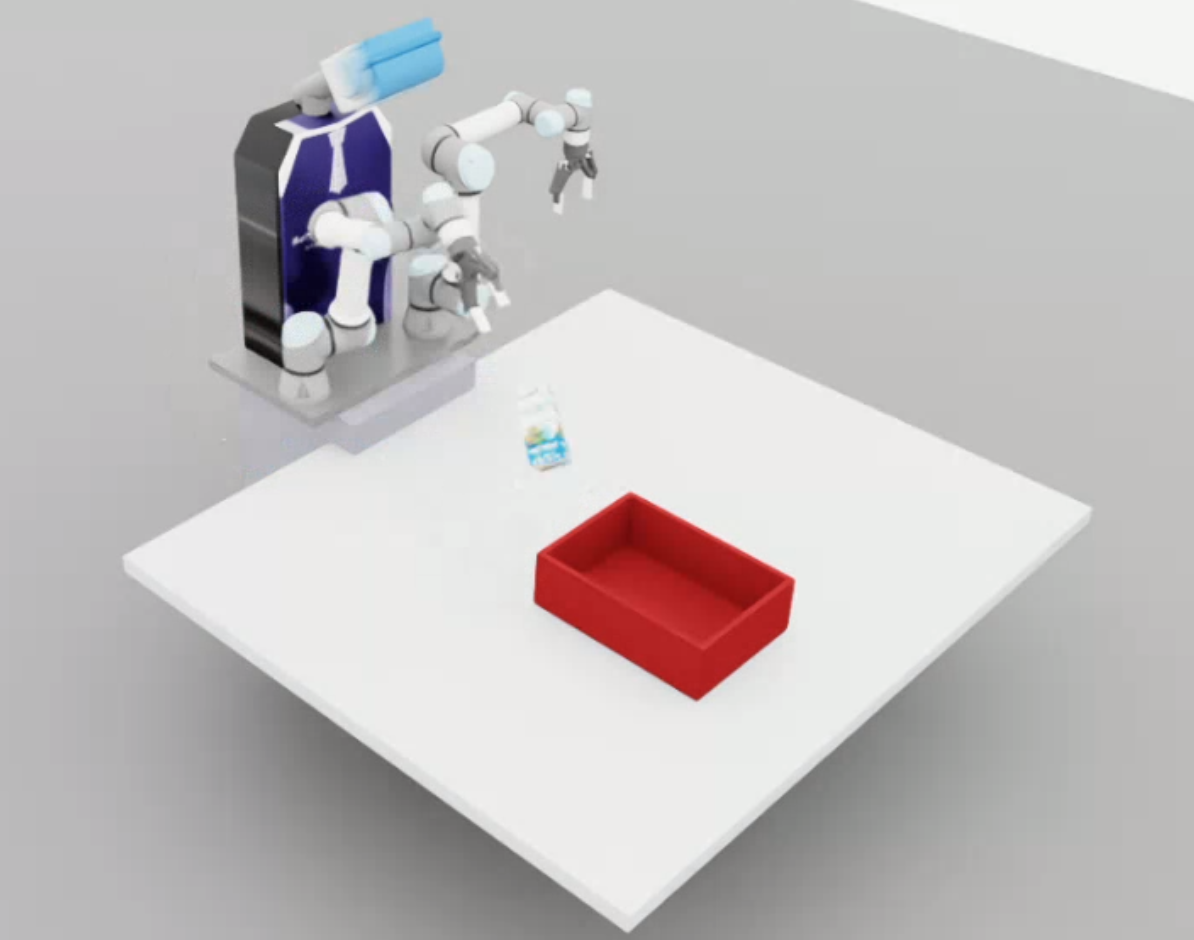
\includegraphics[width=\textwidth]{report_pics/throw_env_1.png}
\caption{Kinematic attachment.}
\label{fig:throw_env_1}
\end{subfigure}
\hfill
\begin{subfigure}{0.31\textwidth}
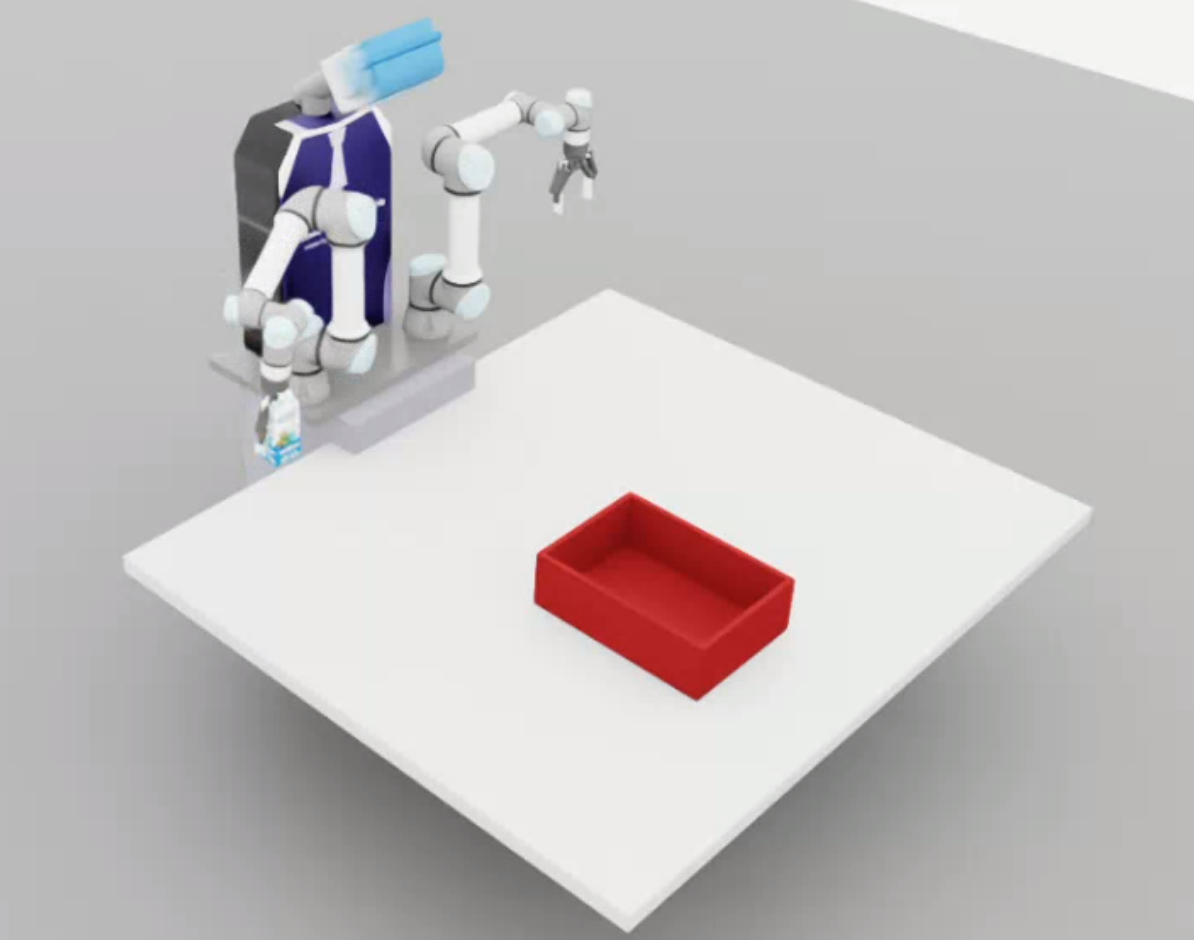
\includegraphics[width=\textwidth]{report_pics/throw_env_2.png}
\caption{Dynamic friction.}
\label{fig:throw_env_2}
\end{subfigure}
\hfill
\begin{subfigure}{0.31\textwidth}
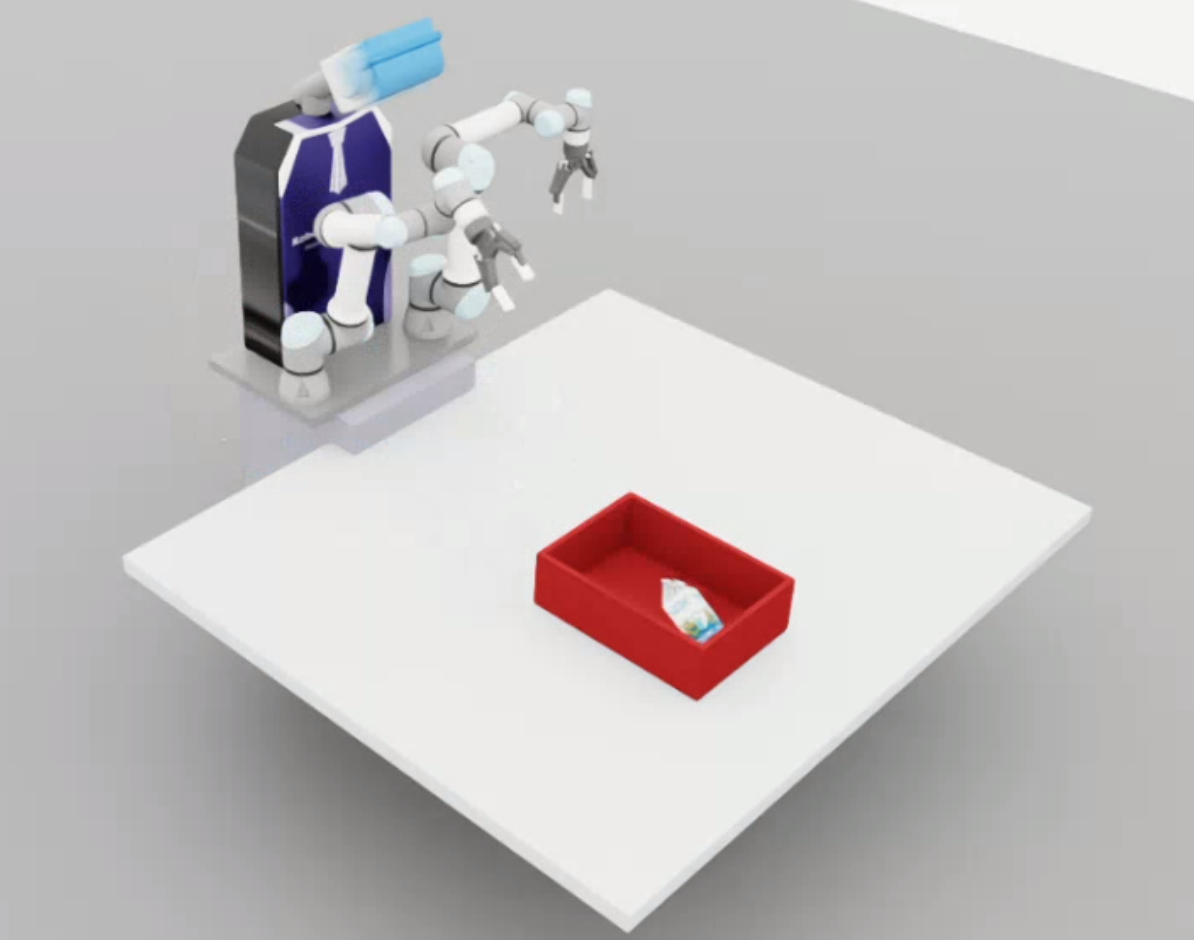
\includegraphics[width=\textwidth]{report_pics/throw_env_3.png}
\caption{During training.}
\label{fig:throw_env_3}
\end{subfigure}
\caption{The throwing environment. The robot stands on a 0.6~m base with a work table and a randomised target basket. Left: kinematic attachment variant. Centre: dynamic friction variant. Right: environment during a training episode with the object attached to the end-effector.}
\label{fig:throw_env}
\end{figure}

The throwing environment (Figure~\ref{fig:throw_env}) targets a 0.5~kg object into a basket randomly positioned on the table, with a success threshold of 0.15~m. The core design challenge is maintaining stability of the object within the gripper under extreme angular velocities during the throwing wind-up: micro-slips between the gripper pads and the object produce unpredictable trajectories that destroy the learning signal.

To address this, two complementary variants were implemented. In the kinematic attachment variant, physical contact is temporarily bypassed: the object follows the end-effector exactly at every simulation step until a velocity threshold of 2.0~m/s is reached, at which point the object is released to a ballistic physics simulation. This deterministic pre-release phase guarantees clean feedback during early learning. In the dynamic friction variant, the object is held purely by contact forces, and the agent must apply continuous torque to maintain grip against centripetal forces---preparing the policy for conditions it would encounter on physical hardware.

The throwing action is structured as four parameters---two shoulder angles, a release timing, and a trajectory duration---mirroring a prior formulation validated on a CPU-bound simulator~\cite{kasaei2023learning}. A streamlined environment variant achieves a 3--5$\times$ speed improvement over the standard path by executing the full throw within a single simulation step.

\begin{figure}[t!]
\centering
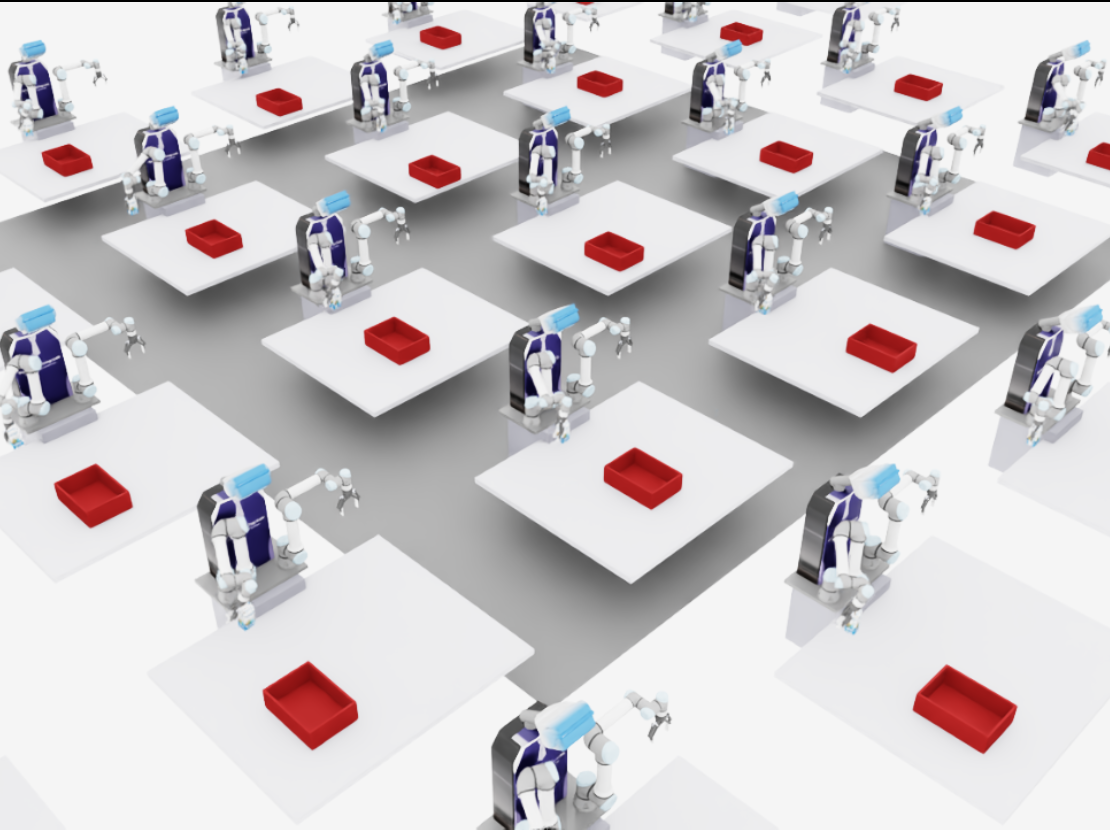
\includegraphics[width=0.7\textwidth]{report_pics/throw_train.png}
\caption{Training progression for the throwing environment, showing reward convergence and success rate over training steps.}
\label{fig:throw_train}
\end{figure}

\begin{figure}[t!]
\centering
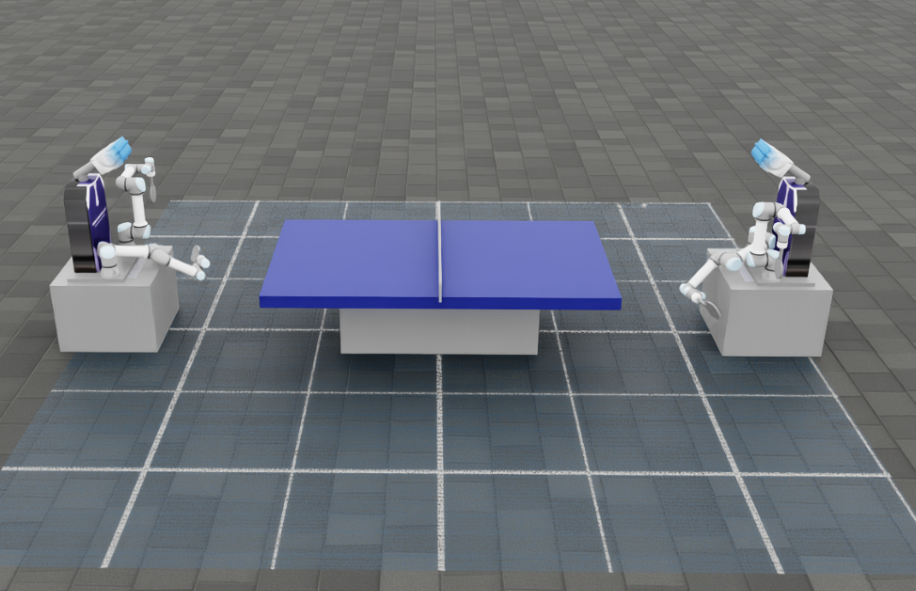
\includegraphics[width=0.48\textwidth]{report_pics/tt_env_1.png}
\caption{The table-tennis environment. Two dual-arm systems with racket attachments compete on a regulation table.}
\label{fig:tt_env_1}
\end{figure}

\subsection{Table Tennis}

The table-tennis environment (Figure~\ref{fig:tt_env_1}) implements a competitive simulation with two identical dual-arm systems at opposite ends of the table. Each robot has a racket attached to the active arm. The environment uses virtual contact detection---computing the distance between the racket surface and the ball at each step---rather than physical contact sensors. The game logic includes table-zone scoring, random ball serves with alternating servers, and a structured reward function that provides feedback for paddle contact, return velocity, opponent-table success, and various penalties.

\subsection{Design Comparison}

Table~\ref{tab:env_comparison} summarises the key differences between the two environments.

\begin{table}[H]
\centering
\caption{Design Comparison of the Two Environments}
\label{tab:env_comparison}
\begin{tabularx}{\textwidth}{@{} l X X @{}}
\toprule
\textbf{Aspect} & \textbf{Throwing} & \textbf{Table Tennis} \\
\midrule
Robot setup & One dual-arm system at origin & Two dual-arm systems at opposite ends \\
End-effector & Two-finger gripper & Racket (fixed joint) \\
Action space & 6 dimensions (per-step) or 4 (macro-action) & 12 dimensions (two 6-D arms) \\
Observation space & 27 dimensions (per-step) or 10 (macro) & 69 dimensions \\
Core mechanic & Kinematic attachment with velocity release & Virtual paddle-ball contact and table zones \\
Reward & Distance-based with success bonus & Contact, velocity, table success, floor penalty \\
\bottomrule
\end{tabularx}
\end{table}

\section{Why GPU-Accelerated Training Matters}
\label{sec:advantage}

\subsection{Training Results}

The defining bottleneck in reinforcement learning is the rate at which the simulator can generate experience. Table~\ref{tab:sim_comparison} compares platforms by their typical output.

\begin{table}[H]
\centering
\caption{Simulation Platforms for Reinforcement Learning}
\label{tab:sim_comparison}
\begin{tabularx}{\textwidth}{@{} l l l c @{}}
\toprule
\textbf{Platform} & \textbf{Physics Engine} & \textbf{Parallelism} & \textbf{Output} \\
\midrule
GPU-accelerated & GPU-native physics & Thousands on one device & $\sim$50,000+ instances/s \\
GPU-based (MJX) & Convex optimisation & Thousands on one device & $\sim$100,000 instances/s \\
CPU-based (Bullet) & Iterative contact (CPU) & Tens per machine & $<$5,000 instances/s \\
CPU-based (ODE) & Iterative contact (CPU) & A few per machine & $\sim$1,000 instances/s \\
\bottomrule
\end{tabularx}
\end{table}

A prior throwing study using a CPU-bound platform trained a policy for 50,000 steps with a single simulation instance, achieving 94\% accuracy~\cite{kasaei2023learning}. The GPU-accelerated implementation presented here reaches 82 million training steps in approximately 14 wall-clock hours on a single compute node---over 1,600 times the step count in comparable time. Figures~\ref{fig:throw_train} and~\ref{fig:tt_train} in Section~\ref{sec:environments} show the training progression for both environments, illustrating how the increased simulation throughput translates directly to faster policy convergence.

HPC benchmarks quantify the scaling behaviour (Table~\ref{tab:scalability}):

\begin{table}[H]
\centering
\caption{Simulation Output at Scale}
\label{tab:scalability}
\begin{tabular}{@{} c c c c @{}}
\toprule
\textbf{Instances} & \textbf{Steps/s (outer)} & \textbf{Steps/s (physics)} & \textbf{Memory (MB)} \\
\midrule
128   & 80.5   & 25,773  & 9.3  \\
1,024 & 571.0  & 182,711 & 17.4 \\
4,096 & 1,806.7 & 578,139 & 45.7 \\
8,192 & 2,650.1 & 848,032 & 82.4 \\
\bottomrule
\end{tabular}
\end{table}

Moving from 128 to 1,024 parallel instances (an 8-fold increase) yields a 7.1-fold output increase, with scaling beginning to plateau at 8,192 instances as the GPU approaches full occupancy. Memory use grows linearly from 9.3 to 82.4~MB, well within a modern GPU's capacity. The streamlined environment path achieves a 1.41$\times$ physics output improvement over the standard path by eliminating per-step software overhead.

\subsection{Physics Fidelity and the Two-Phase Curriculum}

A critical failure mode in learning to throw occurs when the physics simulation cannot maintain stable contact between the gripper and the object during high-velocity motion. Slips produce object trajectories that are uncorrelated with the agent's intended action---destroying the feedback signal that gradient-based methods depend on.

CPU-bound iterative contact solvers are particularly vulnerable to this problem because their temporal resolution between frames is too coarse to capture the high-frequency dynamics of a swinging arm. GPU-native physics mitigates this through parallel sub-stepping: the simulation can run at higher temporal resolution without proportional wall-clock penalties, producing cleaner and more reliable feedback for the learning algorithm.

The two-variant design of the throwing environment is a direct response to this challenge. In the first phase, kinematic attachment guarantees a deterministic pre-release trajectory, enabling the agent to learn the mapping from target position to release parameters without being penalised for grip dynamics it has not yet mastered. In the second phase, the agent must maintain grip under centripetal forces generated by its own trajectories---learning physically realistic constraints rather than exploiting simulation artefacts.

\subsection{Randomisation at Scale}

Bridging the gap between simulation and reality requires training across varied conditions: different friction coefficients, object masses, and target positions. On CPU-bound platforms, each randomised configuration requires a separate simulation process, and scaling to thousands of variations is prohibitively slow. A GPU-accelerated platform simulates thousands of independent randomisation seeds simultaneously at the same wall-clock cost as a single deterministic configuration. This ensures the policy learns robust features rather than overfitting to one set of conditions. In the throwing environment, the target basket position is randomised across episodes; in the table-tennis environment, ball serve velocity, position, and server identity vary.

\begin{figure}[t!]
\centering
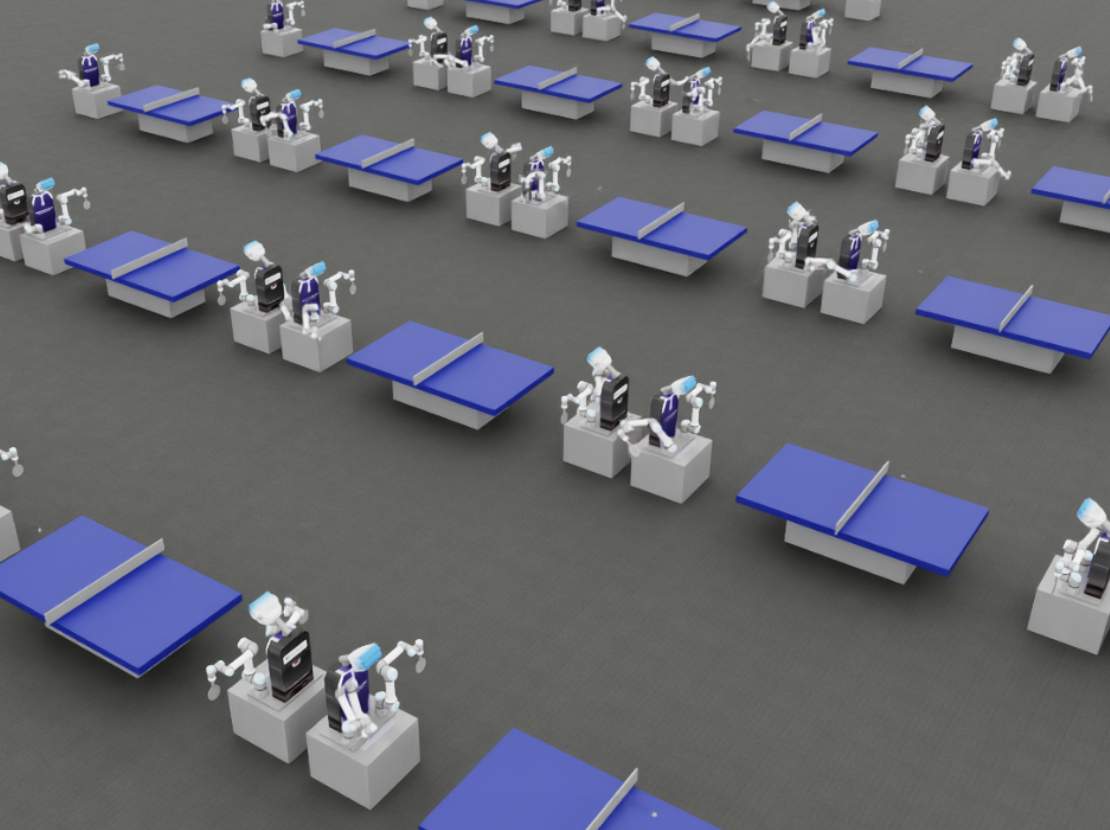
\includegraphics[width=0.7\textwidth]{report_pics/table_tennis_train.png}
\caption{Training progression for the table-tennis environment, showing reward convergence and contact rate over training iterations.}
\label{fig:tt_train}
\end{figure}

\section{Empirical Validation}
\label{sec:validation}

\subsection{Table Tennis}

\begin{figure}[t!]
\centering
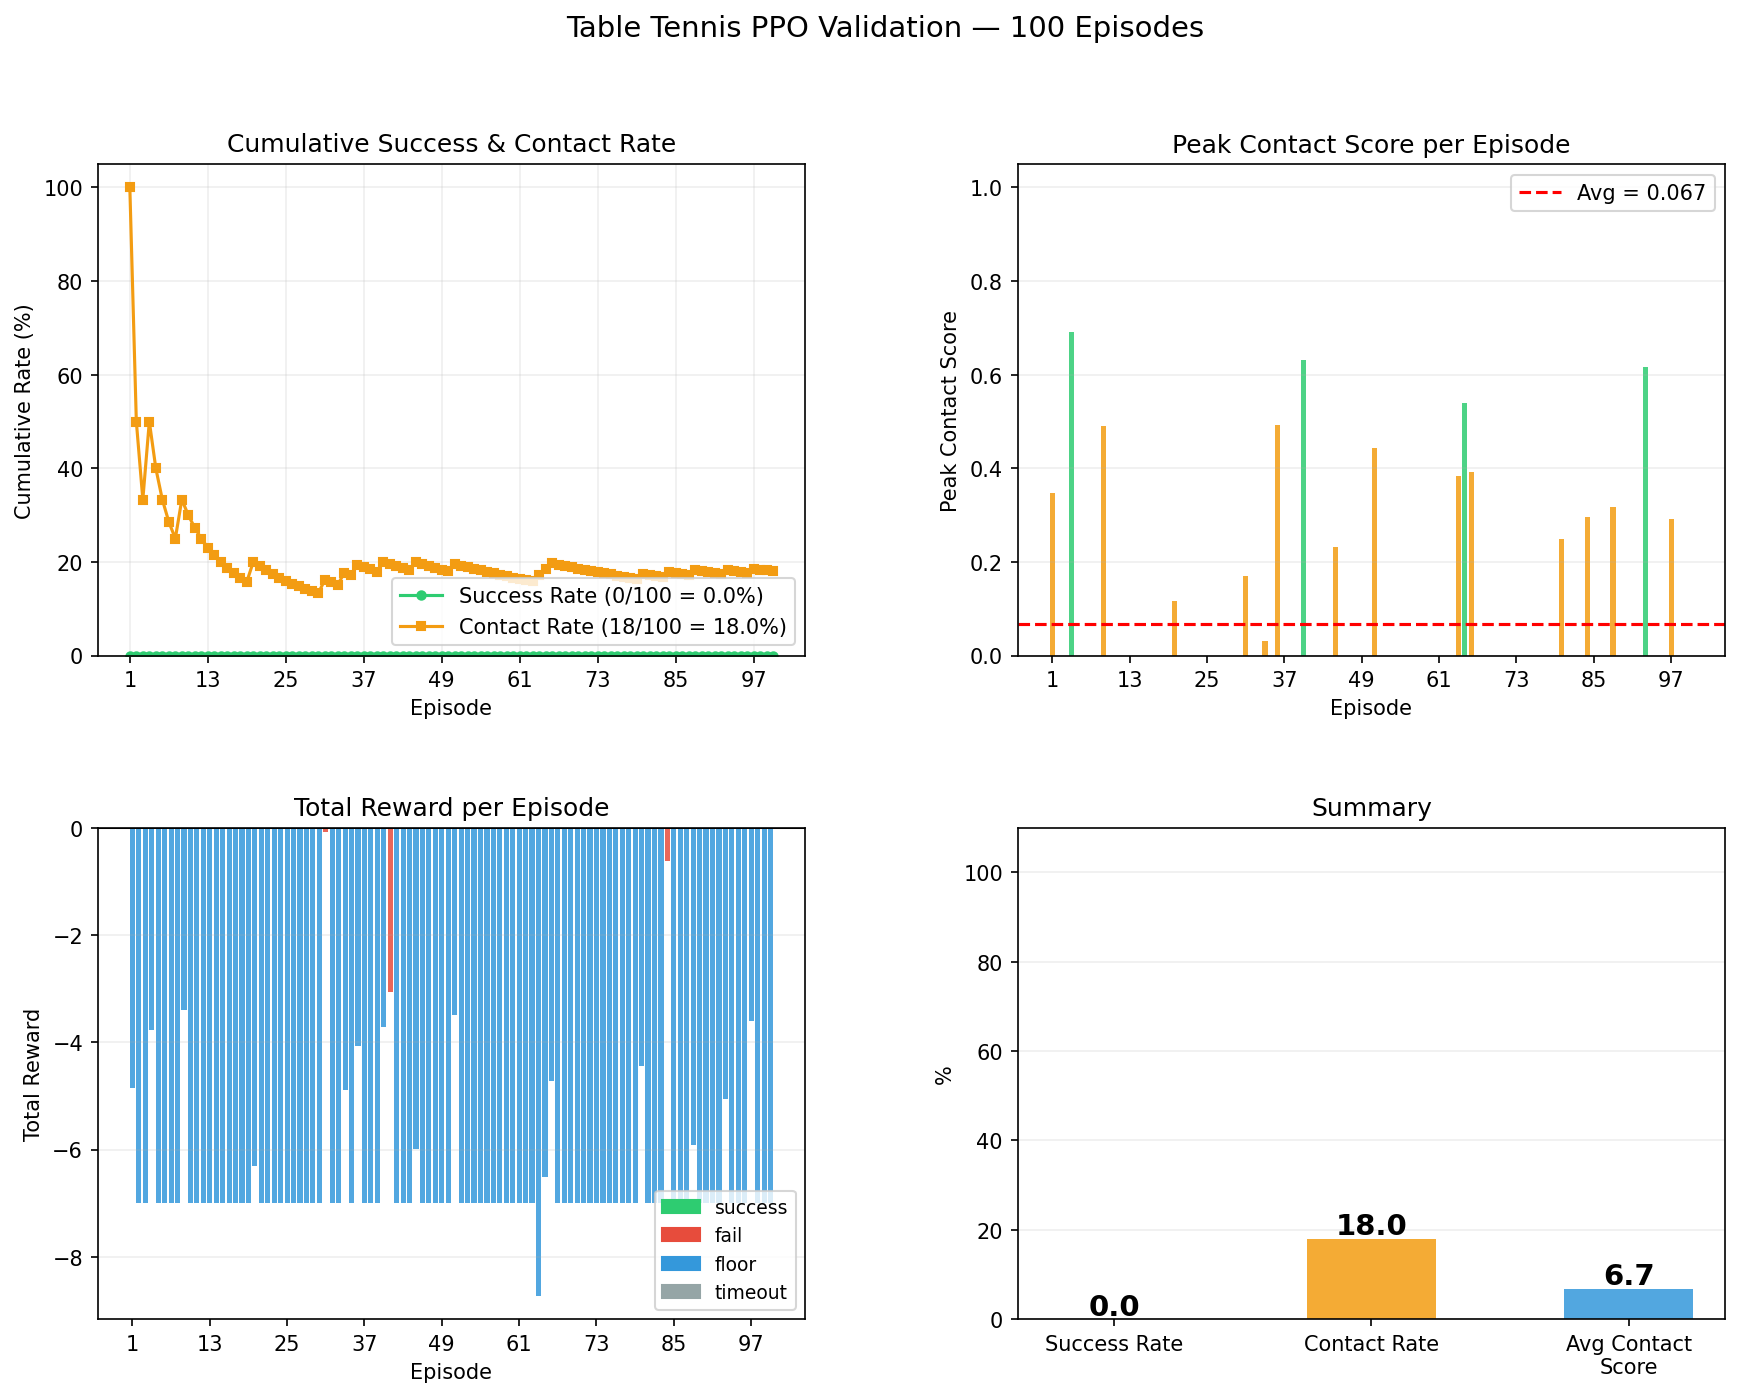
\includegraphics[width=0.7\textwidth]{report_pics/tt_valid.png}
\caption{Table-tennis validation after 130,000 training iterations. Six panels show total reward per episode, reward component breakdown, episode outcomes, and contact quality over time.}
\label{fig:tt_valid}
\end{figure}

A policy trained for 130,000 iterations was evaluated deterministically against 100 serve episodes (Figure~\ref{fig:tt_valid}). Table~\ref{tab:tt_results} summarises the outcomes.

\begin{table}[H]
\centering
\caption{Table-Tennis Validation (130,000 Iterations, 100 Episodes)}
\label{tab:tt_results}
\begin{tabular}{@{} l c c c @{}}
\toprule
\textbf{Metric} & \textbf{Episodes} & \textbf{Rate} & \textbf{Mean Reward} \\
\midrule
Immediate floor drop  & 97 & 97.0\% & $-7.00$ \\
Hits own table        & 3  & 3.0\%  & $-0.53$ \\
Paddle contact made   & 18 & 18.0\% & ---     \\
Reaches opponent zone & 0  & 0.0\%  & ---     \\
\hline
Total                 & 100 & --- & $-6.50$ \\
\bottomrule
\end{tabular}
\end{table}

The 18\% contact rate indicates the policy has begun to approach the incoming ball, with a mean peak contact score of 0.37 across contacted episodes. Most episodes (82\%) ended with the ball immediately hitting the floor without any paddle interaction. At this stage of training, a non-zero contact rate confirms the learning signal is functional; further training is expected to improve return accuracy as the velocity and position-based reward components strengthen.

\subsection{Object Throwing}

\begin{figure}[t!]
\centering
\begin{subfigure}{0.48\textwidth}
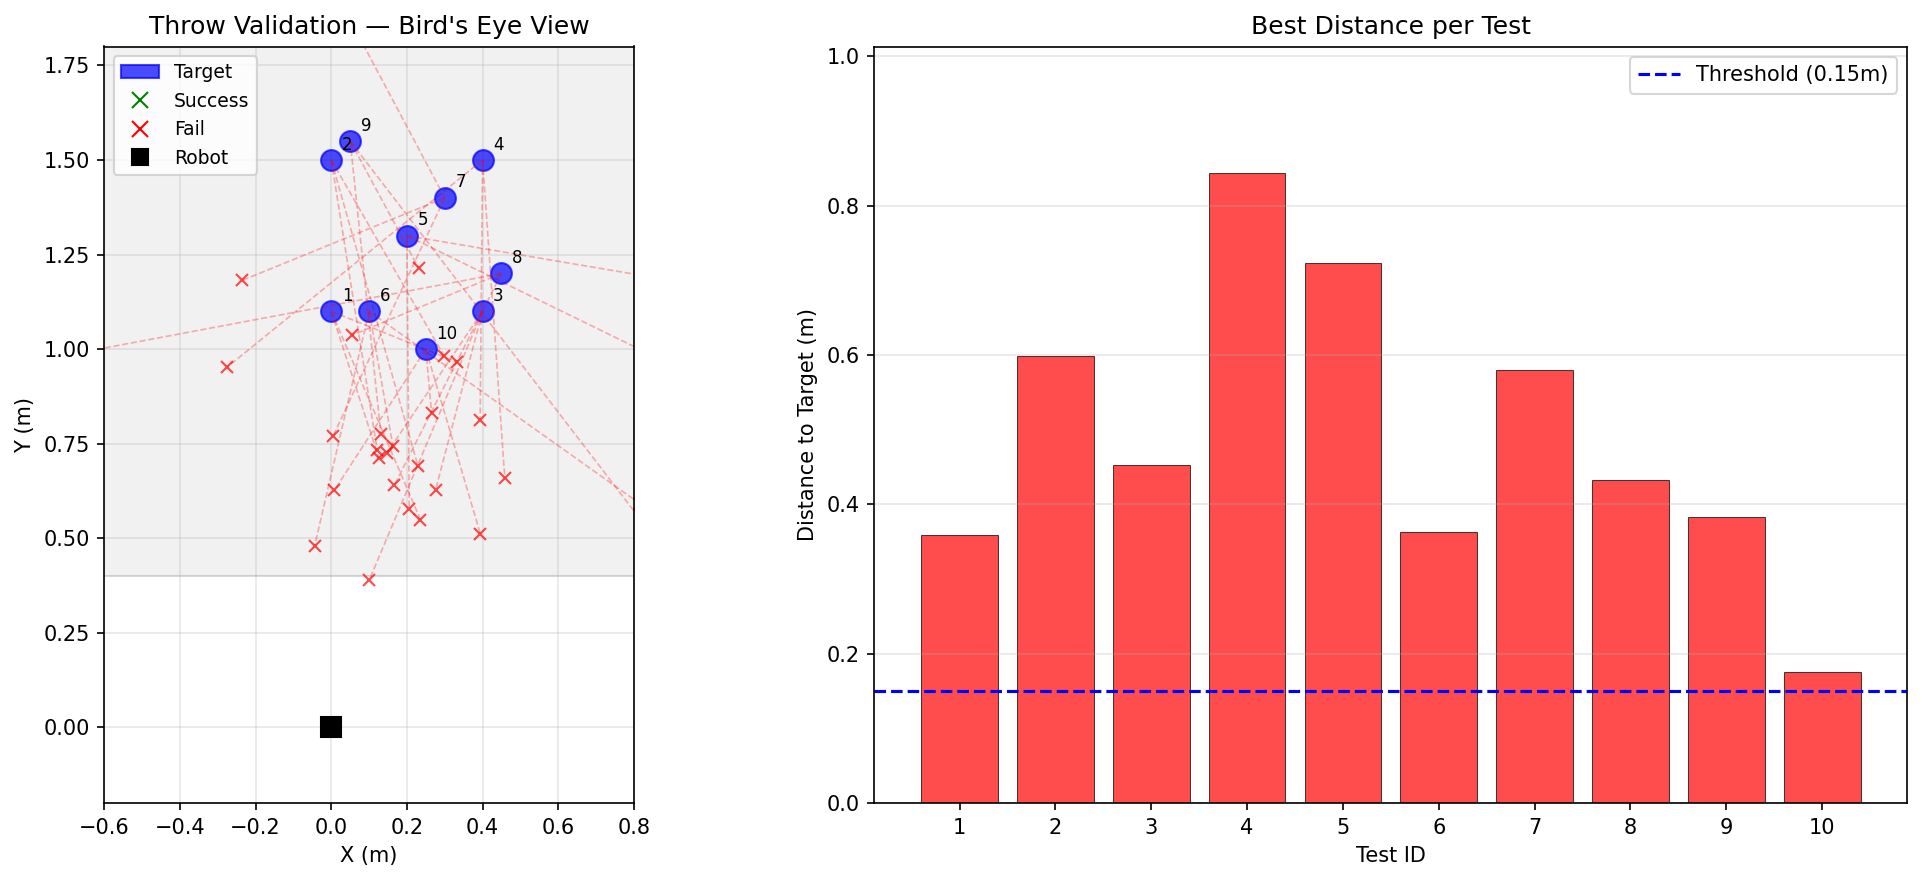
\includegraphics[width=\textwidth]{report_pics/validation_results_SB3-start.png}
\caption{Untrained baseline.}
\label{fig:throw_sb3_start}
\end{subfigure}
\hfill
\begin{subfigure}{0.48\textwidth}
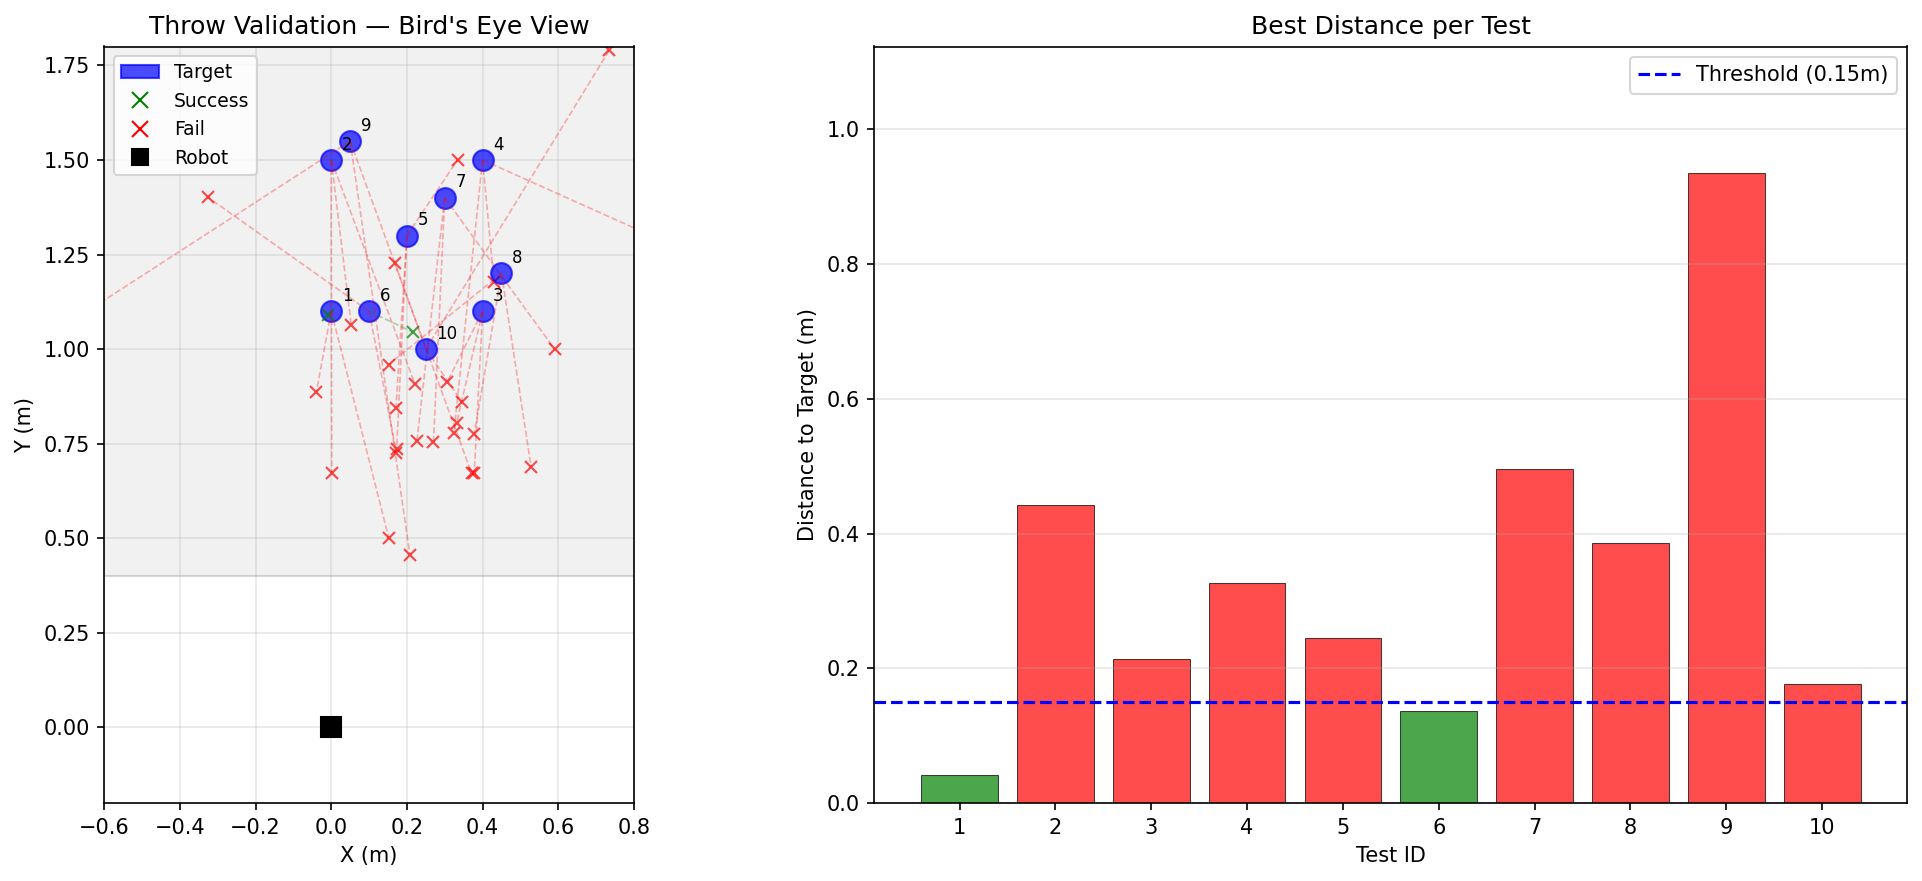
\includegraphics[width=\textwidth]{report_pics/validation_results_SB3-82M.png}
\caption{After 82 million training steps.}
\label{fig:throw_sb3_82M}
\end{subfigure}
\caption{Throwing validation. Ten target positions, three attempts each, 0.15~m success threshold.}
\label{fig:throw_sb3}
\end{figure}

The throwing policy was evaluated against 10 predefined target positions with three attempts each (Figure~\ref{fig:throw_sb3}). Table~\ref{tab:throw_progression} compares the untrained baseline against the trained policy.

\begin{table}[H]
\centering
\caption{Throwing Validation Progression}
\label{tab:throw_progression}
\begin{tabular}{@{} l c c @{}}
\toprule
\textbf{Metric} & \textbf{Untrained} & \textbf{After 82M Steps} \\
\midrule
Targets reached       & 0 / 10 (0.0\%)  & 2 / 10 (20.0\%) \\
Mean best distance    & 0.49~m           & 0.34~m \\
Best single throw     & 0.18~m           & 0.04~m \\
\bottomrule
\end{tabular}
\end{table}

The untrained agent produces near-identical throwing parameters for every target---shoulder angles near 1.2 radians, uniform release timing, and a fixed trajectory duration. After 82 million steps, completed in approximately 14 wall-clock hours, the policy has learned distinct parameters per target and achieved a best throw of 0.04~m. The prior CPU-bound formulation achieved 94\% accuracy after 50,000 steps in its original configuration; the GPU-accelerated implementation trades some per-step sample efficiency for a massive increase in total training output, enabling orders-of-magnitude more environment interactions in comparable wall-clock time.

\section{Conclusion}
\label{sec:conclusion}

This report has presented two deep reinforcement learning environments for dual-arm manipulation, developed on a GPU-accelerated simulation platform. Both environments---throwing and table tennis---achieve training output unattainable on CPU-bound simulators. The throwing environment's two-phase strategy protects the learning signal during early training while preparing policies for realistic contact dynamics. The table-tennis environment provides a functional competitive game pipeline with randomised serves and comprehensive reward decomposition.

The empirical results confirm the approach is viable. The throwing policy improved from a 0.49~m untrained mean distance to a 0.04~m best throw and 20\% target success rate. The table-tennis policy reached an 18\% paddle contact rate. Training benchmarks show 7.1$\times$ scaling and a 1.41$\times$ speedup over the standard environment path.

Limitations include the early stage of policy convergence and the restriction to single-arm control. The primary direction for future work is full dual-arm coordination. The shared robot model and solver infrastructure already support expanding the action space to 12 DOF. Three extensions are planned: bi-manual throwing, where one arm positions the object while the other releases; dual-racket table tennis for simultaneous forehand and backhand coverage; and a coordinated push-grasp task requiring synchronised arm motion. The benchmarking and validation infrastructure deployed on the cluster provides a replicable methodology for measuring training efficiency as the action space scales to full dual-arm coordination.

\bibliographystyle{IEEEtran}
\begin{thebibliography}{99}

\bibitem{plappert2021asymmetric}
M.~Plappert, R.~Houthooft, P.~Dhariwal, S.~Sidor, R.~Y.~Chen, X.~Chen, T.~Asfour, P.~Abbeel, and M.~Andrychowicz,
``Asymmetric self-play for automatic goal discovery in robotic manipulation,''
\textit{arXiv preprint arXiv:2101.04882}, 2021.

\bibitem{sukhbaatar2018learning}
S.~Sukhbaatar, Z.~Lin, I.~Kostrikov, G.~Synnaeve, A.~Szlam, and R.~Fergus,
``Intrinsic motivation and automatic curricula via asymmetric self-play,''
in \textit{International Conference on Learning Representations (ICLR)}, 2018.

\bibitem{mit_pingpong}
D.~B.~D'Ambrosio, J.~Abelian, and S.~K.~Abeyruwan,
``Achieving human level competitive robot table tennis,''
\textit{arXiv preprint arXiv:2408.03906}, 2024.

\bibitem{sony_ace}
Sony Corporation,
``Project Ace: A high-speed robotic arm for table tennis,''
Sony AI Technical Report, 2024.

\bibitem{columbia_tt}
D.~B\"{u}chler, S.~G\"{u}nther, B.~Belousov, and J.~Peters,
``Learning to play table tennis: A study in sim-to-real transfer,''
\textit{IEEE Robotics and Automation Letters}, vol.~7, no.~2, pp.~1872--1879, 2022.

\bibitem{isaac_lab}
M.~Mittal, C.~Yu, Q.~Vuong, F.~Faghihi, H.~X.~Chen, A.~Murali, et~al.,
``Orbit: A unified simulation framework for interactive robot learning environments,''
\textit{IEEE Robotics and Automation Letters}, vol.~8, no.~6, pp.~3740--3747, 2023.

\bibitem{skrl}
SKRL Contributors,
``SKRL---Reinforcement Learning library,''
\url{https://github.com/Toni-SM/skrl}, 2025.

\bibitem{kasaei2023learning}
S.~H.~Kasaei and M.~Kasaei,
``Learning to throw objects with a robot arm using deep reinforcement learning,''
in \textit{Proceedings of the IEEE International Conference on Robotics and Automation (ICRA)}, 2023.

\end{thebibliography}

\end{document}
